\documentclass{article}
% Change "article" to "report" to get rid of page number on title page
\usepackage{amsmath,amsfonts,amsthm,amssymb}
\usepackage{setspace}
\usepackage{Tabbing}
\usepackage{fancyhdr}
\usepackage{lastpage}
\usepackage{extramarks}
\usepackage{chngpage}
\usepackage{soul,color}
\usepackage{graphicx,float,wrapfig}
\usepackage{multirow}

% In case you need to adjust margins:
\topmargin=-0.45in      %
\evensidemargin=0in     %
\oddsidemargin=0in      %
\textwidth=6.5in        %
\textheight=9.0in       %
\headsep=0.25in         %

% Homework Specific Information
\newcommand{\hmwkTitle}{Weekly Report II}
\newcommand{\hmwkClass}{}
\newcommand{\hmwkAuthorName}{Donglai\ Wei}


% Setup the header and footer
\pagestyle{fancy}                                                       %
\lhead{\hmwkAuthorName}                                                 %
\rhead{\firstxmark}                                                     %
\lfoot{\lastxmark}                                                      %
\cfoot{}                                                                %
\rfoot{Page\ \thepage\ of\ \pageref{LastPage}}                          %
\renewcommand\headrulewidth{0.4pt}                                      %
\renewcommand\footrulewidth{0.4pt}                                      %

% This is used to trace down (pin point) problems
% in latexing a document:
%\tracingall

%%%%%%%%%%%%%%%%%%%%%%%%%%%%%%%%%%%%%%%%%%%%%%%%%%%%%%%%\begin{enumerate}

% Some tools
\newcommand{\enterProblemHeader}[1]{\nobreak\extramarks{#1}{#1 continued on next page\ldots}\nobreak%
                                    \nobreak\extramarks{#1 (continued)}{#1 continued on next page\ldots}\nobreak}%
\newcommand{\exitProblemHeader}[1]{\nobreak\extramarks{#1 (continued)}{#1 continued on next page\ldots}\nobreak%
                                   \nobreak\extramarks{#1}{}\nobreak}%

\newlength{\labelLength}
\newcommand{\labelAnswer}[2]
  {\settowidth{\labelLength}{#1}%
   \addtolength{\labelLength}{0.25in}%
   \changetext{}{-\labelLength}{}{}{}%
   \noindent\fbox{\begin{minipage}[c]{\columnwidth}#2\end{minipage}}%
   \marginpar{\fbox{#1}}%

   % We put the blank space above in order to make sure this
   % \marginpar gets correctly placed.
   \changetext{}{+\labelLength}{}{}{}}%

\setcounter{secnumdepth}{0}
\newcommand{\homeworkProblemName}{}%
\newcounter{homeworkProblemCounter}%
\newenvironment{homeworkProblem}[1][Problem \arabic{homeworkProblemCounter}]%
  {\stepcounter{homeworkProblemCounter}%
   \renewcommand{\homeworkProblemName}{#1}%
   \section{\homeworkProblemName}%
   \enterProblemHeader{\homeworkProblemName}}%
  {\exitProblemHeader{\homeworkProblemName}}%

\newcommand{\problemAnswer}[1]
  {\noindent\fbox{\begin{minipage}[c]{\columnwidth}#1\end{minipage}}}%

\newcommand{\problemLAnswer}[1]
  {\labelAnswer{\homeworkProblemName}{#1}}

\newcommand{\homeworkSectionName}{}%
\newlength{\homeworkSectionLabelLength}{}%
\newenvironment{homeworkSection}[1]%
  {% We put this space here to make sure we're not connected to the above.
   % Otherwise the changetext can do funny things to the other margin

   \renewcommand{\homeworkSectionName}{#1}%
   \settowidth{\homeworkSectionLabelLength}{\homeworkSectionName}%
   \addtolength{\homeworkSectionLabelLength}{0.25in}%
   \changetext{}{-\homeworkSectionLabelLength}{}{}{}%
   \subsection{\homeworkSectionName}%
   \enterProblemHeader{\homeworkProblemName\ [\homeworkSectionName]}}%
  {\enterProblemHeader{\homeworkProblemName}%

   % We put the blank space above in order to make sure this margin
   % change doesn't happen too soon (otherwise \sectionAnswer's can
   % get ugly about their \marginpar placement.
   \changetext{}{+\homeworkSectionLabelLength}{}{}{}}%

\newcommand{\sectionAnswer}[1]
  {% We put this space here to make sure we're disconnected from the previous
   % passage

   \noindent\fbox{\begin{minipage}[c]{\columnwidth}#1\end{minipage}}%
   \enterProblemHeader{\homeworkProblemName}\exitProblemHeader{\homeworkProblemName}%
   \marginpar{\fbox{\homeworkSectionName}}%

   % We put the blank space above in order to make sure this
   % \marginpar gets correctly placed.
   }%

%%%%%%%%%%%%%%%%%%%%%%%%%%%%%%%%%%%%%%%%%%%%%%%%%%%%%%%%%%%%%



%%%%%%%%%%%%%%%%%%%%%%%%%%%%%%%%%%%%%%%%%%%%%%%%%%%%%%%%%%%%%
% Make title
\title{\vspace{0.3in}\textmd{\textbf{\hmwkTitle}}}
\date{2010.4.21}
\author{\textbf{\hmwkAuthorName}}
%%%%%%%%%%%%%%%%%%%%%%%%%%%%%%%%%%%%%%%%%%%%%%%%%%%%%%%%%%%%%

\begin{document}
\begin{spacing}{1.1}
\maketitle



  
\section{1. Generalized Formula}
\subsection{1.0  ME Algorithm settings} 
\large {\bf 0) Notation:}\\
 \underline{Observations:}\\
  $\ \ \vec x=(x^{(1)},...,x^{(N)})$  \\
 \underline{Hidden Variables}:\\
  $\ \ \vec z=(z^{(1)},...,z^{(N)})$: assignments from stochastic process;\\    
  $\ \ \theta$: parameter from exponential distribution;\\ 
 \underline{Hyperparameters}:\\
 $\ \ \lambda$:($\lambda_{0},\lambda_{a}$ for $\theta$ and $\alpha,\gamma$ for $\vec z$) \\ \\
The goal is to find the log probability: $log(p(\vec x|\lambda))=log(\sum_{\vec z} [\int_\theta \! p(\vec x,\vec z,\theta|\lambda) \, d\theta])$\\ \\
\large {\bf 1) $\theta$:}\\
For Exponential Family,we can integrate out $\theta$ in close form: \\ \\
likelihood of the data:$\ \ \ \ \ \ \ \ \ \ \ \ \ \ \ \ \ \ \ \ p(x|\theta)=v(x)exp\{\sum_{a \in \mathcal{A}} \theta_{a}\phi_{a}(x)-\Phi(\theta) \}$ \\ 
Prior for the parameter:$\ \ \ \ \ \ \ \ \ \ \ \ \ \ \ \ \   p(\theta|\lambda)=exp\{\sum_{a\in\mathcal{A}} \theta_{a}\lambda_{0}\lambda_{a}-\lambda_{0}\Phi_(\theta)-\Omega(\lambda) \}$\\ 
Posterior for the parameter :$\ \ \ \ \ \ \ \ \ \ \ p(\theta|x^{(1)},...,x^{(N)},\lambda)=p(\theta|\bar \lambda)$ \\
where $ \bar \lambda_{0}=\lambda_{0}+N,\bar \lambda_{a}=\frac{\lambda_{0}\lambda_{a}+\sum_{l=1}^{N}\phi_{a}(x^{(l)})}{\lambda_{0}+N}\lambda_{0}+N $\\
Thus, $\theta$ can be easily integrate out:
$\ log(p(x^{(1)},...,x^{(N)}|\lambda))=\Omega(\bar \lambda)-\Omega(\lambda)+\sum_{l=1}^{N}v(x^{(l)})$\\ \\
\large {\bf 2) $\vec z$:}\\
But the discrete variable $\vec z$ is hard to sum out.\\
So instead, we pick the MAP estimator $\vec z^{*}$:\\
\begin{eqnarray*}
 log(p(\vec x|\lambda))
& = & log(\sum_{\vec z} [\int_\theta \! p(\vec x,\vec z,\theta|\lambda) \, d\theta]) \\
& \approx & log(\int_\theta \! p(\vec x,\vec z^{*},\theta|\lambda) \, d\theta) \\
& = &  log(\int_\theta \! p(\vec x,\theta|\vec z^{*},\lambda) \, d\theta)+log( p(\vec z|\lambda)) \\
& = &  \Omega(\bar \lambda)-\Omega(\lambda)+\sum_{l=1}^{N}v(x^{(l)})+log( p(\vec z|\lambda))
\end{eqnarray*}
 


\subsection{1.1  $\theta$: Conjugated Exponential Family}
K: number of clusters in $\vec z$ \\   
N: number of observations\\ 
$N_{c}$: the number of points in cluster c\\ 
\subsubsection*{a)Nomal-Inverse-Wishart}
\begin{eqnarray*} 
p(\theta|\lambda)
&=& p(\mu,\Sigma|m_{0},\eta_{0},\xi_{0},B_{0}) \\
&=&NIW(m_{0},\eta_{0},\xi_{0},B_{0}) \\
&=& \frac{1}{Z}\lvert\Sigma\lvert^{-((\eta_{0}+d)/2+1)}exp(-\frac{1}{2}tr(B_{0}\Sigma^{-1})-\frac{\xi_{0}}{2}(\mu-m_{0})^{T}\Sigma^{-1}(\mu-m_{0}))
\end{eqnarray*}
$Z=\dfrac{2^{\eta_{0}d/2}\Gamma_{D}(\eta_{0}/2)(2\pi/\xi)^{d/2}}{\lvert\Sigma\lvert^{\eta_{0}/2}},$\\
$\Gamma_{D}(x)=\pi^{\frac{D(D-1)}{4}}\Pi_{i=1}^{D}\Gamma(x+\frac{1-i}{2})$

\begin{eqnarray*} 
log(p(\vec x,\theta|\vec z, \lambda))
& = & log(p(\theta|\lambda))+\sum_{n=1}^{N}[log(p(x_{n}|z_{n},\theta))]\\ 
& = & log(\mathcal{N}(\mu|m_{0},\xi_{0}\Omega)\mathcal{W}(\Omega|\eta_{0},B_{0}))+\sum_{n=1}^{N}[log(\mathcal{N}(x_{n}|z_{n},\mu,\Omega))]\\ 
& = & -\frac{DN}{2}log(2\pi)+log(\mathcal{N}(\mu|m_{c},\xi_{c}\Omega_{c})\mathcal{W}(\Omega_{c}|\eta_{c},B_{c}))+log(p(\vec x|\vec z, \lambda)) \\
\end{eqnarray*}
$S_{c}$: the covariance of datas in cluster c\\ 
$\phi_{c}=\phi_{0}+N_{c}$\\
$m_{c}=\frac{N_{c}\bar x_{c}+\xi_{0}m_{0}}{\xi_{c}}$\\
$B_{c}=B_{0}+N_{c}S_{c}+\frac{N_{c}\xi_{0}}{\xi_{c}}(\bar x_{c}-m_{0})(\bar x_{c}-m_{0})^{T}$\\
$\eta_{c}=\eta_{0}+N_{c}$\\
$\xi_{c}=\xi_{0}+N_{c}$\\ \\ \\
$log(\int_\theta \! p(\vec x,\theta|\vec z,\lambda) \, d\theta)$\\
\begin{eqnarray*} 
& = & -\frac{DN}{2}log(2\pi)+log(\int_\theta \! \mathcal{N}(\mu|m_{c},\xi_{c}\Omega_{c})\mathcal{W}(\Omega_{c}|\eta_{c},B_{c}) \, d\theta)+log( p(\vec x|\vec z, \lambda))\\
& = & -\frac{DN}{2}log(2\pi)+0+\sum_{c=1}^{K}log(Z(\bar \lambda_{c}))-log(Z( \lambda_{c}))\\
& = & -\frac{DN}{2}log(2\pi)+\sum_{c=1}^{K}log(\dfrac{2^{\eta_{c}D/2}\Gamma_{D}(\eta_{c}/2)(2\pi/\xi_{c})^{D/2}\lvert\Sigma\lvert^{\eta_{0}/2}}{2^{\eta_{0}D/2}\Gamma_{D}(\eta_{0}/2)(2\pi/\xi_{0})^{D/2}\lvert\Sigma\lvert^{\eta_{c}/2}})\\ 
& = & -\frac{DN}{2}log(2\pi)+\sum_{c=1}^{K}[\frac{DN}{2}log(2)-(\frac{D}{2}log\frac{\xi_{c}}{\xi_{0}})+(\frac{\eta_{0}}{2}log det(B_{0})
-\frac{\eta_{c}}{2}log det(B_{c}))+(log \frac{\Gamma_{D}(\frac{\eta_{c}}{2})}{\Gamma_{D}(\frac{\eta_{0}}{2})})]
\end{eqnarray*}

\subsubsection*{b)Dirichlet-Multinomial}
\begin{eqnarray*} 
p(\theta|\lambda)
&=& \mathcal{D}(\beta|\phi_{0}) \\
&=& \frac{1}{Z}\Pi_{i=1}^{i=K}\beta_{i}^{(\phi_{0}-1)}\\
Z=\dfrac{\Gamma(\phi_{0})^{K}}{\Gamma(K\phi_{0})}
\end{eqnarray*}
\begin{eqnarray*} 
p(\vec x,\theta|\vec z, \lambda)
&=&\Pi_{n=1}^{N}[p(x_{n}|z_{n},\theta)]p(\theta|\lambda) \\
&=&\Pi_{n=1}^{N}[\mathcal{M}(x_{n}|z_{n},\alpha)] \times \mathcal{D}(\alpha|\phi_{0}) \\
&=&\mathcal{D}(\alpha|\phi_{c})\times p(\vec x|\vec z, \lambda) \\
\phi_{c}=\phi_{0}+N_{c}
\end{eqnarray*}
\begin{eqnarray*} 
log(\int_\theta \! p(\vec x,\theta|\vec z,\lambda) \, d\theta)
&=& log(\int_\theta \! \mathcal{D}(\alpha|\phi_{c})\, d\theta)+log(p(\vec x|\vec z, \lambda)) \\
&=& 0+log(Z(\phi_{c}))-log(Z(\phi_{0}))\\
&=& log(\frac{\Pi_{c=1}^{K}\Gamma(\phi_{c})}{\Gamma(N+K\phi_{0})}/\frac{\Gamma(\phi_{0})^{K}}{\Gamma(K\phi_{0})})\\ \\
&=& log(\frac{\Gamma(K\phi_{0})}{\Gamma(N+K\phi_{0})})+\sum_{c=1}^{K}log(\frac{\Gamma(\phi_{c})}{\Gamma(\phi_{0})})
\end{eqnarray*}

\subsection{1.2  $\vec z$: Stochastic Process}
\subsubsection*{a)DP mixture(with Chinese Restaurant Process)}
\begin{center}
 Graphical Model for DP mixture\\
    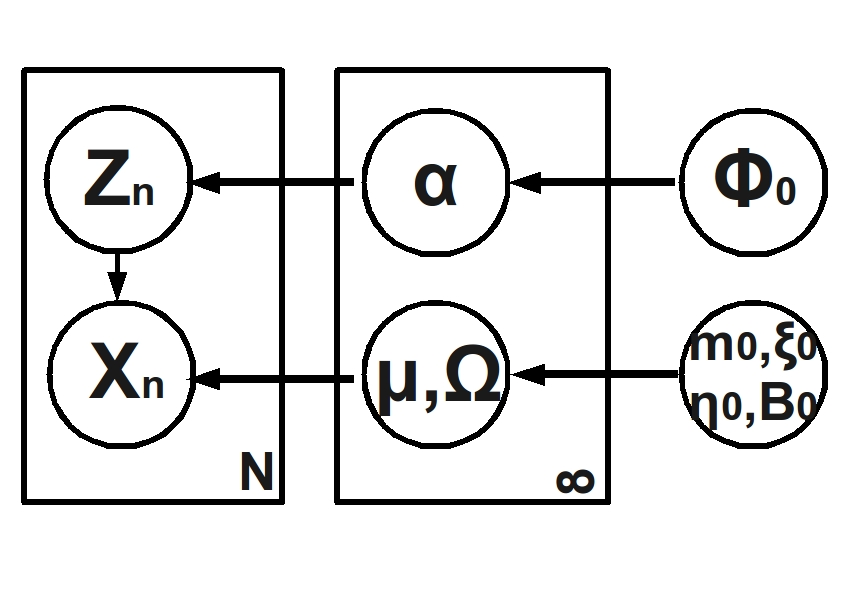
\includegraphics[width=3in,height=2in]{dp.jpg} 
\end{center}
K: number of clusters in $\vec z$ \\   
N: number of observations\\ 
$N_{c}$: the number of points in cluster c\\ 
$p(\vec z|\lambda)=p(z_{1},...,z_{N}|\phi_{0})=\Pi_{j=1}^{j=N}p(z_{j}|z_{1},...,z_{j-1},\phi_{0})$\\ \\
$p(z_{j}|z_{1},...,z_{j-1},\phi_{0})=\sum_{k=1}^{K(j)}\frac{m_{k(j)}}{j-1+\phi_{0}}\delta_{z_{j}=k}+\frac{\phi_{0}}{j-1+\phi_{0}}\delta_{z_{j}=K(j)+1}$\\ \\
1) Partition:$\Pi_{j=1}^{j=N}\frac{1}{\phi_{0}+j-1}=\frac{\Gamma(\phi_{0})}{\Gamma(N+\phi_{0})}$\\ 
2) Forming new clusters:$\phi_{0}^{K}$\\ 
3) Accumulating for all clusters:$\Pi_{j=1}^{j=N}(N_{j}-1)!=\Pi_{j=1}^{j=N}\Gamma(N_{j})$\\ \\
So,$p(\vec z|\lambda)=\frac{\Gamma(\phi_{0})}{\Gamma(N+\phi_{0})}\Pi_{c=1}^{K}[\Gamma(N_{c})]\phi_{0}^{K}$
\subsubsection*{b)HDP(with Chinese Franchise Process)}
Notation:\\ \\
1) Global: J Restaurants, K global dishes, T tables, N datas,\\
$t_{ji}:$ the table that customer i in Restaurant j sits;\\
$k_{jt}:$ the dish that table t in Restaurant j serves;\\
$\vec k:$ new dish different from what has been served;\\
$\vec t:$ the table different from what has been occupied;\\
2) Counting so far (during the process)\\
$m_{jk}:$ number of tables in Restaurant j serving dish k;\\
$m_{.k}:$ number of tables serving dish k;\\
$m_{j.}:$ number of tables in Restaurant j;\\
$m_{..}:$ number of tables;\\
$n_{jtk}:$ number of customers in Restaurant j at table t eating dish k;\\
$n_{jt.}:$ number of customers in Restaurant j at table t;\\
$n_{j..}:$ number of customers in Restaurant j;\\ \\
$p(\vec z,\vec k|\lambda)=p(k_{11},...,k_{JT_{J}}|\gamma)p(t_{11},...,t_{JN_{J}}|\alpha)$\\ \\
$p(k_{11},...,k_{JT_{J}}|\gamma)=\Pi_{j=1}^{J}(\Pi_{i=1}^{T_{j}}p(k_{ji}|\vec k_{1},...\vec k_{j-1},k_{j1},...,k_{j(i-1)},\gamma))$\\ \\
$p(t_{11},...,t_{JN_{J}}|\alpha)=\Pi_{j=1}^{J}(\Pi_{i=1}^{N_{j}}p(t_{ji}|t_{j1},...,t_{j(i-1)},\alpha))$\\ \\
$p(k_{jt}|\vec k_{1},...\vec k_{j-1},k_{j1},...,k_{j(t-1)},\gamma)=\sum_{k=1}^{K}\frac{m_{.k}}{m_{..}-1+\gamma}\delta_{k_{jt}=k}+\frac{\gamma}{m_{..}-1+\gamma}\delta_{k_{ji}=\vec k}$\\ \\
$p(t_{ji}|t_{j1},...,t_{j(i-1)},\alpha)=\sum_{t=1}^{m_{j.}}\frac{n_{jt.}}{i-1+\alpha}\delta_{t_{ji}=t}+\frac{\alpha}{i-1+\alpha}\delta_{t_{ji}=\vec t}$\\ \\

1) Partition:\\
k:\ $\Pi_{w=1}^{\sum_{j=1}^{J}m_{j.}}\frac{1}{\gamma+w-1}=\Pi_{w=1}^{m_{..}}\frac{1}{\gamma+w-1}=\frac{\Gamma(\gamma)}{\Gamma(T+\gamma)}$\\ 
t:\ $\Pi_{j=1}^{J}\Pi_{i=1}^{i=n_{j..}}\frac{1}{\alpha+i-1}=\Pi_{j=1}^{j=J}\frac{\Gamma(\alpha)}{\Gamma(n_{j..}+\alpha)}$\\ 

2) Forming new clusters (1st point in the cluster): \\
k: \ $\gamma^{K}$\\ 
t: \ $\Pi_{j=1}^{J}\alpha^{m_{j.}}$\\ 

3) Accumulating for each clusters (other points in the cluster): \\
k: \ $\Pi_{k=1}^{k=K}(m_{.k}-1)!=\Pi_{k=1}^{k=K}\Gamma(m_{.k})$\\ 
t: \ $\Pi_{j=1}^{j=J}\Pi_{t=1}^{t=m_{j.}}(n_{jt.}-1)!=\Pi_{j=1}^{j=J}\Pi_{t=1}^{t=m_{j.}}\Gamma(n_{jt.})$\\ 

So,$log(p(\vec z,\vec k|\lambda))=log\{\Pi_{j=1}^{J}[\frac{\Gamma(\alpha)}{\Gamma(n_{j..}+\alpha)}\Pi_{t=1}^{m_{j.}}(\Gamma(n_{jt.}))]\alpha^{\sum_{j=1}^{J}m_{j.}}\}
 +log\{\frac{\Gamma(\gamma)}{\Gamma(T+\gamma)}\Pi_{k=1}^{K} [\Gamma(m_{.k})] \gamma^{K}\}$

\begin{center}
Graphical Model for HDP\\
    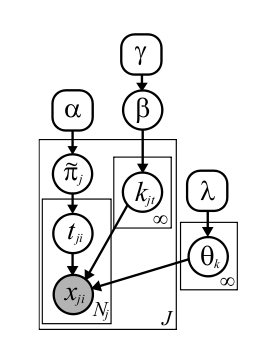
\includegraphics[width=4in,height=5in]{hdp.jpg} 
\end{center}




\end{spacing}
\end{document}

%%%%%%%%%%%%%%%%%%%%%%%%%%%%%%%%%%%%%%%%%%%%%%%%%%%%%%%%%%%%%
